Before we get to subfigures, let's start with an ordinary figure (see \autoref{fig:apparatus}).
Most publications do not include a List of Figures; the inclusion of the List of Figures (as required by the Graduate School Style Guide) requires attention to certain details.
For example, the default behaviour is for the entire caption to be listed as the figure title in the List of Figures.
However, since informative captions are almost invariably to long to be appropriate for the List of Figures, a short title can be specified as an optional argument to the $\backslash$\texttt{caption} command; if specified, the short title will be used in the List of Figures.
If the short title is specified but empty, the figure will not be included in the list of figures.
Notice how \autoref{fig:apparatus} has a long caption.
However, if you look it up in the List of Figures, you will see that it has a tastefully short caption there.

\begin{figure}
\centering %
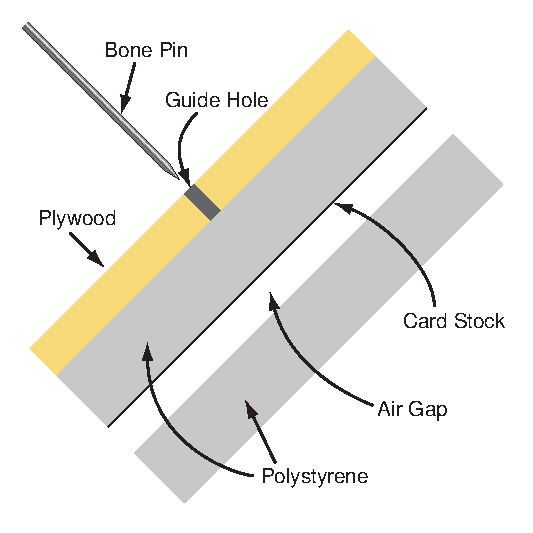
\includegraphics{figures/Apparatus}%
\caption[Experimental task setup]{%
  Experimental task setup (0.5$\times$ scale).  A slab of polystyrene is laminated with card stock and separated from a second slab by an air gap. The pin's direction of movement is guided by a drill-hole through the covering plywood layer.
}%
\label{fig:apparatus} %
\end{figure}

So a basic figure is not hard.
But when you want to illustrate a process over time (in this two-dimensional medium), you really need to be able to create a figure that has several subfigures arranged in a row.
Like in \autoref{fig:taskSteps}.

You may also want to refer to a subfigure within a figure (e.g., \autoref{subfig:taskProgress}).

\begin{figure}
\centering %
\subfloat[Start]{%
\label{subfig:taskStart}%

\includegraphics[width=0.275\columnwidth]{figures/TaskStart}%
}%
\hspace{-0.035\columnwidth}%
\subfloat[Carving]{%
\label{subfig:taskProgress}%

\includegraphics[width=0.275\columnwidth]{figures/TaskProgress}%
}%
\hspace{-0.035\columnwidth}%
\subfloat[Complete]{%
\label{subfig:taskComplete}%

\includegraphics[width=0.275\columnwidth]{figures/TaskComplete}%
}%
\hspace{-0.035\columnwidth}%
\subfloat[Failed]{%
\label{subfig:taskFailed}%

\includegraphics[width=0.275\columnwidth]{figures/TaskFailed}%
}%
\caption[Task procedure]{%
  Task procedure.  \subref{subfig:taskStart} The task starts with the tip of the pin resting on the surface of the polystyrene. \subref{subfig:taskProgress} The subject must drive the sharpened pin through the first polystyrene slab.  \subref{subfig:taskComplete} The subject must stop before the pin touches the second slab. \subref{subfig:taskFailed} If the pin penetrates the second slab, the task is failed.
}%
\label{fig:taskSteps}
\end{figure}
